\setcounter{section}{3}


\section{Lecture 4:Jan 27}


\subsection*{Last time}
\begin{itemize}
\item Column space and Nullspace (JM Appendix A)
\item Simple Linear Regression (JF Chapter 5)
\end{itemize}


\subsection*{Today}
\begin{itemize}
\item HW1 posted, due Feb 12th
\item Simple Linear Regression (JF Chapter 5)

\end{itemize}

\subsection*{Least squares estimates}

The simple linear regression (SLR) model writes:
$$
y_i = \beta_0 + \beta_1 x_i + \epsilon_i.
$$

The least squares estimates minimizes the sum of squared error (SSE)  which is 
$$
SS[E] = \sum\limits_{1}^{n}\left( y_i - (\hat{\beta}_0 + \hat{\beta}_1 x_i) \right)^2 = \sum\limits_{1}^{n}(y_i - \hat{y}_i)^2 = \sum\limits_{1}^{n}\epsilon_i^2.
$$
The {\bf least squares} (LS) estimates (in vector form):
$$
\hat{\beta}_{ls} = \left(
\begin{array}{l}
\hat{\beta}_0\\
\hat{\beta}_1\\
\end{array}
\right) =
\left(
\begin{array}{c}
\bar{y} - \hat{\beta}_1 \bar{x}\\
\frac{\sum(x_i - \bar{x})(y_i - \bar{y})}{\sum(x_i - \bar{x})^2}\\
\end{array}
\right).
$$

{\it Definition: } The line satisfying the equation
$$
y = \hat{\beta}_0 + \hat{\beta}_1 x
$$
is called the \underline{linear regression} of $y$ on $x$ which is also called the \underline{least squares line}.

\subsection*{SLR Model in Matrix Form}

\begin{equation*}
\left[ \begin{array}{c} y_1\\ y_2 \\ \vdots \\ y_n\\ \end{array} \right] =
\left[ \begin{array}{c} \beta_0 + \beta_1 x_1\\ \beta_0 + \beta_1 x_2 \\ \vdots \\ \beta_0 + \beta_1 x_n\\ \end{array} \right] +
\left[ \begin{array}{c} \epsilon_1\\ \epsilon_2 \\ \vdots \\ \epsilon_n\\ \end{array} \right]
\end{equation*}

\begin{equation*}
\left[ \begin{array}{c} y_1\\ y_2 \\ \vdots \\ y_n\\ \end{array} \right] =
\left[ \begin{array}{cc} 1   &x_1\\ 1 & x_2 \\ \vdots & \vdots \\ 1 & x_n\\ \end{array} \right] \left[ \begin{array}{c} \beta_0\\ \beta_1 \\ \end{array} \right] +
\left[ \begin{array}{c} \epsilon_1\\ \epsilon_2 \\ \vdots \\ \epsilon_n\\ \end{array} \right]
\end{equation*}

\subsubsection*{Jargons}
\begin{itemize}
  \item $\vecc{X}$  is called the {\it design matrix}
  \item $\vecc{\beta}$ is the vector of parameters
  \item $\epsilon$ is the error vector
  \item $\vecc{Y}$ is the response vector.
\end{itemize}

\subsubsection*{The Design Matrix}

\begin{equation*}
\vecc{X}_{n \times 2} = \left[ \begin{array}{cc} 1   &x_1\\ 1 & x_2 \\ \vdots & \vdots \\ 1 & x_n\\ \end{array} \right]
\end{equation*}

\subsubsection*{Vector of Parameters}

\begin{equation*}
\vecc{\beta}_{2 \times 1} =\left[ \begin{array}{c} \beta_0\\ \beta_1 \\ \end{array} \right] 
\end{equation*}

\subsubsection*{Vector of Error terms}

\begin{equation*}
\vecc{\epsilon}_{n \times 1} =\left[ \begin{array}{c} \epsilon_1\\ \epsilon_2 \\ \vdots \\ \epsilon_n\\ \end{array} \right]
\end{equation*}

\subsubsection*{Vector of Responses}

\begin{equation*}
\vecc{Y}_{n \times 1} =\left[ \begin{array}{c} y_1\\ y_2 \\ \vdots \\ y_n\\ \end{array} \right]
\end{equation*}

\subsubsection*{Gramian Matrix}

\begin{equation*}
\vecc{X}\transpose\vecc{X} =\left[ \begin{array}{cc} n & \sum_i x_i\\ \sum_i x_i  & \sum_i x_i^2\\ \end{array} \right]
\end{equation*}

Therefore, we have

$$
\vecc{Y} = \vecc{X\beta} + \vecc{\epsilon}.
$$

Assume the Gramian matrix has full rank (which actually should be the case, why?), we want to show that 
$$
\hat{\beta}_{ls} = (\vecc{X}\transpose\vecc{X})^{-1}\vecc{X}\transpose\vecc{Y}.
$$
%
The inverse of the Gramian matrix is
$$
 (\vecc{X}\transpose\vecc{X})^{-1} = \frac{1}{n\sum_i(x_i - \bar{x})^2} \left[ \begin{array}{cc} \sum_i x_i^2 & -\sum_i x_i\\ -\sum_i x_i  & n\\ \end{array} \right]
$$
%
Now we have
\begin{equation*}
\begin{aligned}
\hat{\beta}_{ls}
=& (\vecc{X}\transpose\vecc{X})^{-1}\vecc{X}\transpose\vecc{Y}\\=&
  \frac{1}{n\sum_i(x_i - \bar{x})^2} \left[ \begin{array}{cc} \sum_i x_i^2 & -\sum_i x_i\\ -\sum_i x_i  & n\\ \end{array} \right] \left[ \begin{array}{c} \vecc{1}_n\transpose \\ \vecc{x}\transpose\\ \end{array} \right] \vecc{y} \\
=& \frac{1}{n\sum_i(x_i - \bar{x})^2} \left[ \begin{array}{cc} \sum_i x_i^2 & -\sum_i x_i\\ -\sum_i x_i  & n\\ \end{array} \right]  \left[ \begin{array}{c} \sum_i{y_i}\\ \sum_i{x_i y_i} \\ \end{array} \right] \\
=& \frac{1}{n\sum_i(x_i - \bar{x})^2} \left[ \begin{array}{c} (\sum_i x_i^2)(\sum_i y_i) -(\sum_i x_i)(\sum_i x_i y_i)\\ n\sum_i{x_i y_i} - (\sum_i x_i)(\sum_i y_i) \\ \end{array} \right]  \\
= & \left[
\begin{array}{c}
\bar{y} - \frac{\sum(x_i - \bar{x})(y_i - \bar{y})}{\sum(x_i - \bar{x})^2}\ \bar{x}\\
\frac{\sum(x_i - \bar{x})(y_i - \bar{y})}{\sum(x_i - \bar{x})^2}\\
\end{array}
\right]
\end{aligned}
\end{equation*}

\medskip

Some properties:
\begin{itemize}
  \item (a) $\sum{x_i \hat{\epsilon}_i} = 0$.
  \item (b) $\sum{\hat{y}_i \hat{\epsilon}_i} = 0$ (HW1).
\end{itemize}

{\it Proof:} 
For (a), we look at
$$
\begin{aligned}
&\vecc{X}\transpose \vecc{\hat{\epsilon}} \\
=& \vecc{X}\transpose (\vecc{Y - X\hat{\beta}}) \\
=& \vecc{X}\transpose [\vecc{Y} - \vecc{X} (\vecc{X}\transpose\vecc{X})^{-1}\vecc{X}\transpose \vecc{Y}] \\
=& \vecc{X}\transpose \vecc{Y} - \vecc{X}\transpose \vecc{X} (\vecc{X}\transpose\vecc{X})^{-1}\vecc{X}\transpose \vecc{Y} \\
=& \vecc{X}\transpose \vecc{Y} - \vecc{X}\transpose \vecc{Y}\\
=& \vecc{0}
\end{aligned}
$$


{\bf Other quantities in Matrix Form }
\subsubsection*{Fitted values}
$$
\hat{\vecc{Y}} = \left[ \begin{array}{c} \hat{y}_1\\ \hat{y}_2 \\ \vdots \\ \hat{y}_n\\ \end{array} \right] =  \left[ \begin{array}{c} \hat{\beta}_0 + \hat{\beta}_1 x_1\\  \hat{\beta}_0 + \hat{\beta}_1 x_2 \\ \vdots \\  \hat{\beta}_0 + \hat{\beta}_1 x_n\\ \end{array} \right]
=  \left[ \begin{array}{cc} 1   &x_1\\ 1 & x_2 \\ \vdots & \vdots \\ 1 & x_n\\ \end{array} \right] \left[ \begin{array}{c} \hat{\beta}_0\\ \hat{\beta}_1 \\ \end{array} \right]  = X\hat{\beta}
$$

\subsubsection*{Hat matrix}
$$
\begin{aligned}
\hat{\vecc{Y}} =& \vecc{X \hat{\beta}}\\
\hat{\vecc{Y}} =& \vecc{X} (\vecc{X}\transpose\vecc{X})^{-1}\vecc{X}\transpose\vecc{Y}\\
\hat{\vecc{Y}} =& \vecc{HY}\\
\end{aligned}
$$
%
where $\vecc{H} = \vecc{X} (\vecc{X}\transpose\vecc{X})^{-1}\vecc{X}\transpose$ is called ``hat matrix'' because it turns $\vecc{Y}$ into $\hat{\vecc{Y}}$.

\subsection*{Davis's data example}
For Davis's data, we have
\begin{equation*}
\begin{aligned}
n &= 101 \\
\bar{y} &= \frac{5780}{101} = 57.228\\
\bar{x} &= \frac{5731}{101} = 56.743\\
\sum(x_i - \bar{x})(y_i - \bar{y}) &= 4435.9\\
\sum(x_i - \bar{x})^2 &= 4539.3,\\
\end{aligned}
\end{equation*}
so that
\begin{equation*}
\begin{aligned}
\hat{\beta}_1 &= \frac{4435.9}{4539.3} = 0.97722\\
\hat{\beta}_0 &= 57.228 - 0.97722 \times 56.743 = 1.7776\\
\end{aligned}
\end{equation*}

Figure~\ref{fig:updatedWeights} shows Davis's data on the measured and reported weight in kilograms of $101$ women who were engaged in regular exercise.
\begin{figure}[H]
\begin{center}
  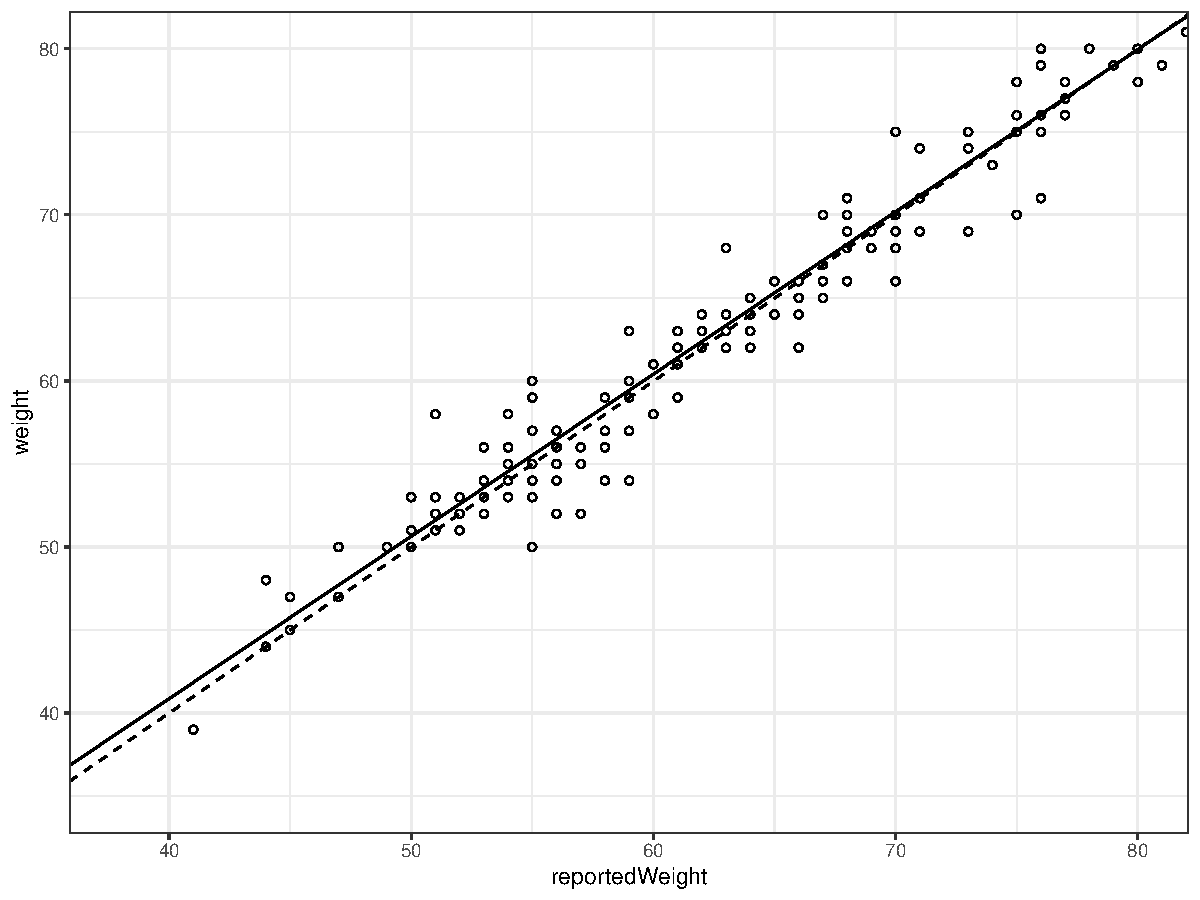
\includegraphics[width=0.8\textwidth]{Lecture3/figure_5_1.pdf}
%  \captionsetup{labelformat=empty}
  \caption{Scatterplot of Davis's data on the measured and reported weight of $101$ women.  The dashed line gives $y = x$.  The solid line gives the least squares line $y = \hat{\beta}_0 + \hat{\beta}_1 x$.}
  \label{fig:updatedWeights}
\end{center}
\end{figure}


